\documentclass[a4paper, 11pt]{article}
\usepackage{geometry}
\usepackage{comment} % enables the use of multi-line comments (\ifx \fi) 
%\usepackage{lipsum} %This package just generates Lorem Ipsum filler text. 
\usepackage{fullpage} % changes the margin
\usepackage{cite}
\usepackage{graphicx}
\usepackage{titlesec}



\geometry{left=1.5cm, right=1.5cm, top=1.5cm, bottom=1.5cm}
\titlespacing*{\section} {0pt}{5pt}{5pt}
\titlespacing*{\subsection} {0pt}{4pt}{4pt}


\begin{document}
%Header-Make sure you update this information!!!!

\begin{center}
    \Large{\textbf{CS200A Final Project Report: Visualizing the World}} \\
    \vspace{0.7cm}
    \large{\today} \\
    \vspace{0.3cm}
    \large{\textbf{Tianxiao Hu, Sheng Shen}}
\end{center}

%\vspace{-0.5cm}

\section*{Introduction}
Image classification is increasingly attracting
attentions. In this project, we leveraged 1,501 images in 20 classes for exploring this problem from the view of machine learning and deep learning. Specifically, we tried to apply the manual crafted feature in various sklearn-based models (such as LR, SVM, KNN and Random Forest). Moreover, we detailed the feature selection process with visualizing its distribution over each class. We finally introduce a CNN-based neural network for comparison, where we find an interesting correlation between regularization and the model's generalizability.

\section*{Data Cleaning}
We were given 1501 pictures containing 20 classes of objects, most of which are RGB images. For gray scale images, we turned them into RGB images during preprocessing. We found files in \texttt{airplanes} folder were corrupted so we replaced the folder with correct data. We also noticed that images have both ``.jpg'' and ``.png'' file extensions, with different size for each picture.

We use \texttt{scikit-learn} \cite{scikit-learn} in our implementation. Other packages and version info are: \texttt{skimage=0.14.0, opencv=3.4.3, tensorflow=1.9}

\section*{Feature Engineering and EDA}
We carefully selected 19 features. Descriptions are listed in Table ~\ref{tab:feature}.

\begin{table}[!htb]
\begin{center}
\begin{tabular}{r|l}
\hline
\textbf{Feature Name}         & \textbf{Description} \\ \hline
size          & picture size (width $\times$ height for grayscale image, width $\times$ height $\times$ 3 for \\
& RGB image) \\ \hline
avg\_red      & mean value of red channel                   \\ \hline
avg\_green    & mean value of green channel                    \\ \hline
avg\_blue     & mean value of blue channel                    \\ \hline
std\_red      & standard derivation of red channel                    \\ \hline
std\_green    & standard derivation of green channel                    \\ \hline
std\_blue     & standard derivation of blue channel                    \\ \hline
avg\_gray     & mean value of grayscale                     \\ \hline
aspect\_ratio & aspect ratio of the image, i.e., the height divided by the width of the image      \\ \hline
harris        & amount of corners detected by Harris corner detector~\cite{harris1988}   \\ \hline
dog           & the differences of images processed by two Gaussian filters with different \\
& variance\\ \hline
avg\_y        & mean value of luminance (Y)     \\ \hline
avg\_cb       & mean value of blue chroma component (Cb)  \\ \hline
avg\_cr       & mean value of red chroma component (Cr)  \\ \hline
std\_y        & standard derivation of luminance (Y)  \\ \hline
std\_cb       & standard derivation of blue chroma component (Cb)                \\ \hline
std\_cr       & standard derivation of red chroma component (Cr) \\ \hline
avg\_hog      & mean value of Histogram of Oriented Gradients (HOG)\cite{hog}              \\ \hline
std\_hog      & standard derivation of Histogram of Oriented Gradients (HOG)               \\ \hline
\end{tabular}
\end{center}
\caption{\label{tab:feature} Features used in classification and description.}
\end{table}

During EDA process, we found two features appeared to be quite interesting: ``avg\_y'' and ``aspect\_ratio'':

\begin{figure}[!h]
\centering
\begin{minipage}[t]{0.48\textwidth}
\centering
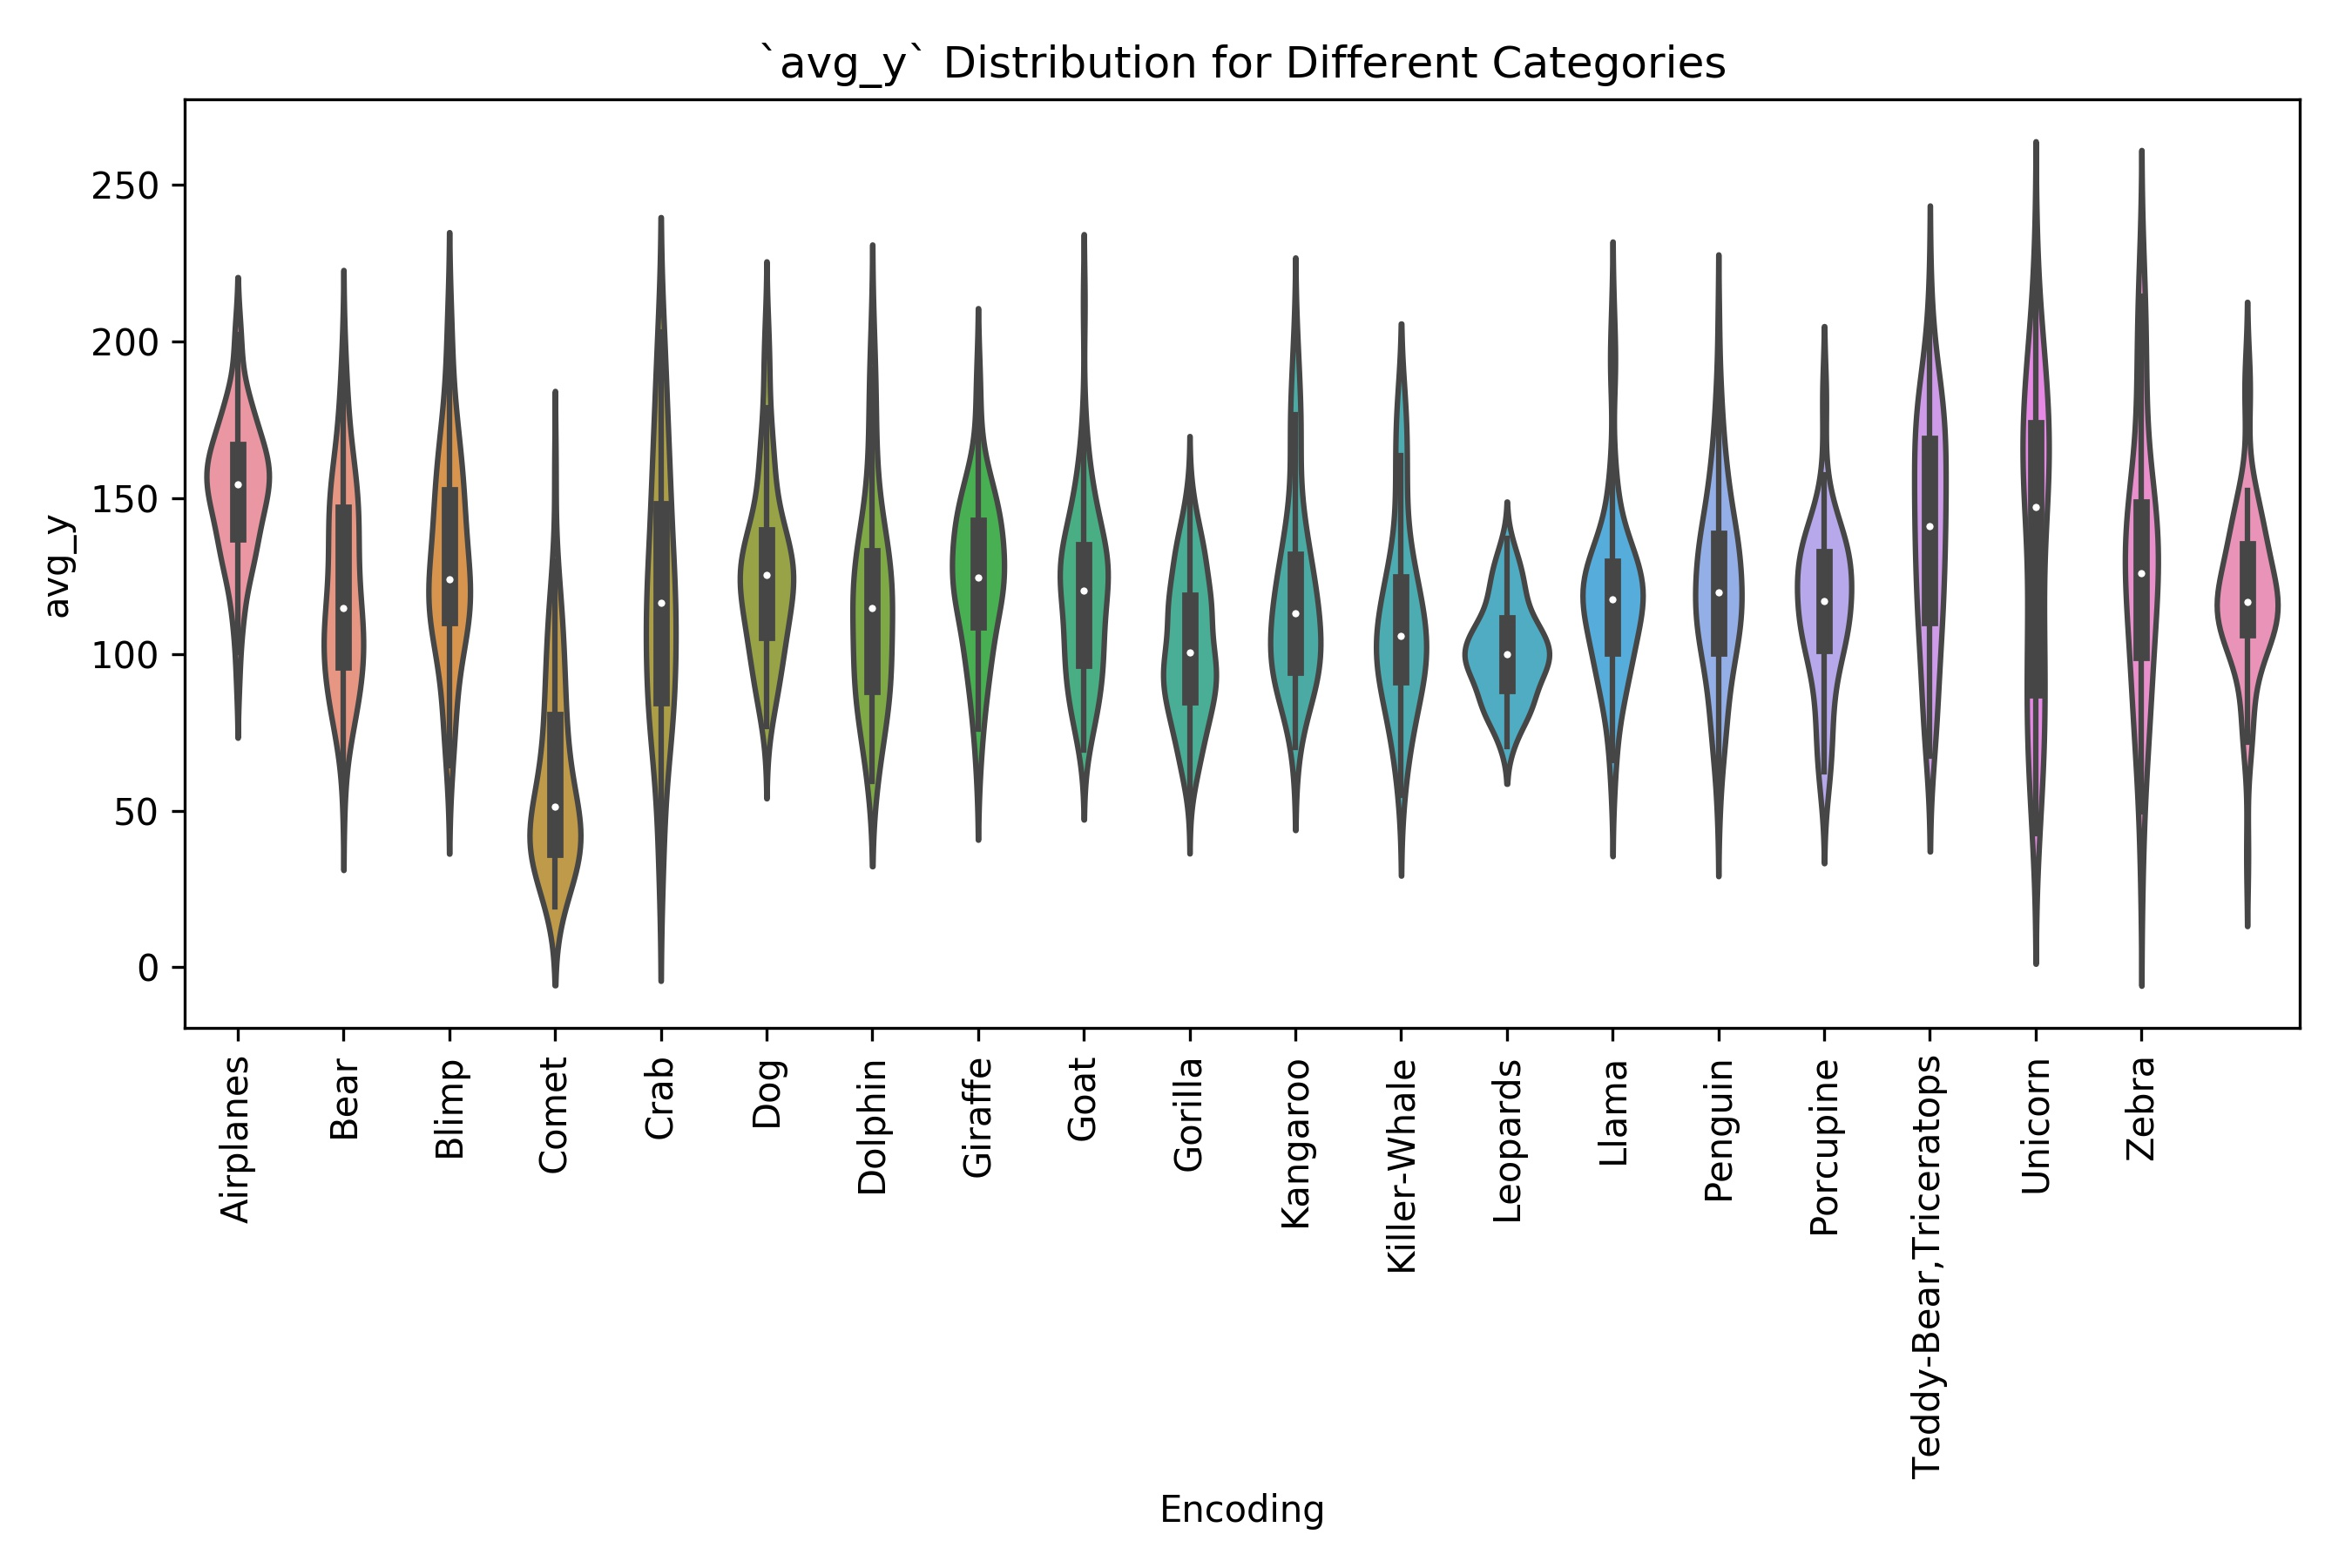
\includegraphics[width=8cm]{image/avg_y.jpg}
\caption{\label{fig:avg_y}EDA of ``avg\_y''}
\end{minipage}
\begin{minipage}[t]{0.48\textwidth}
\centering
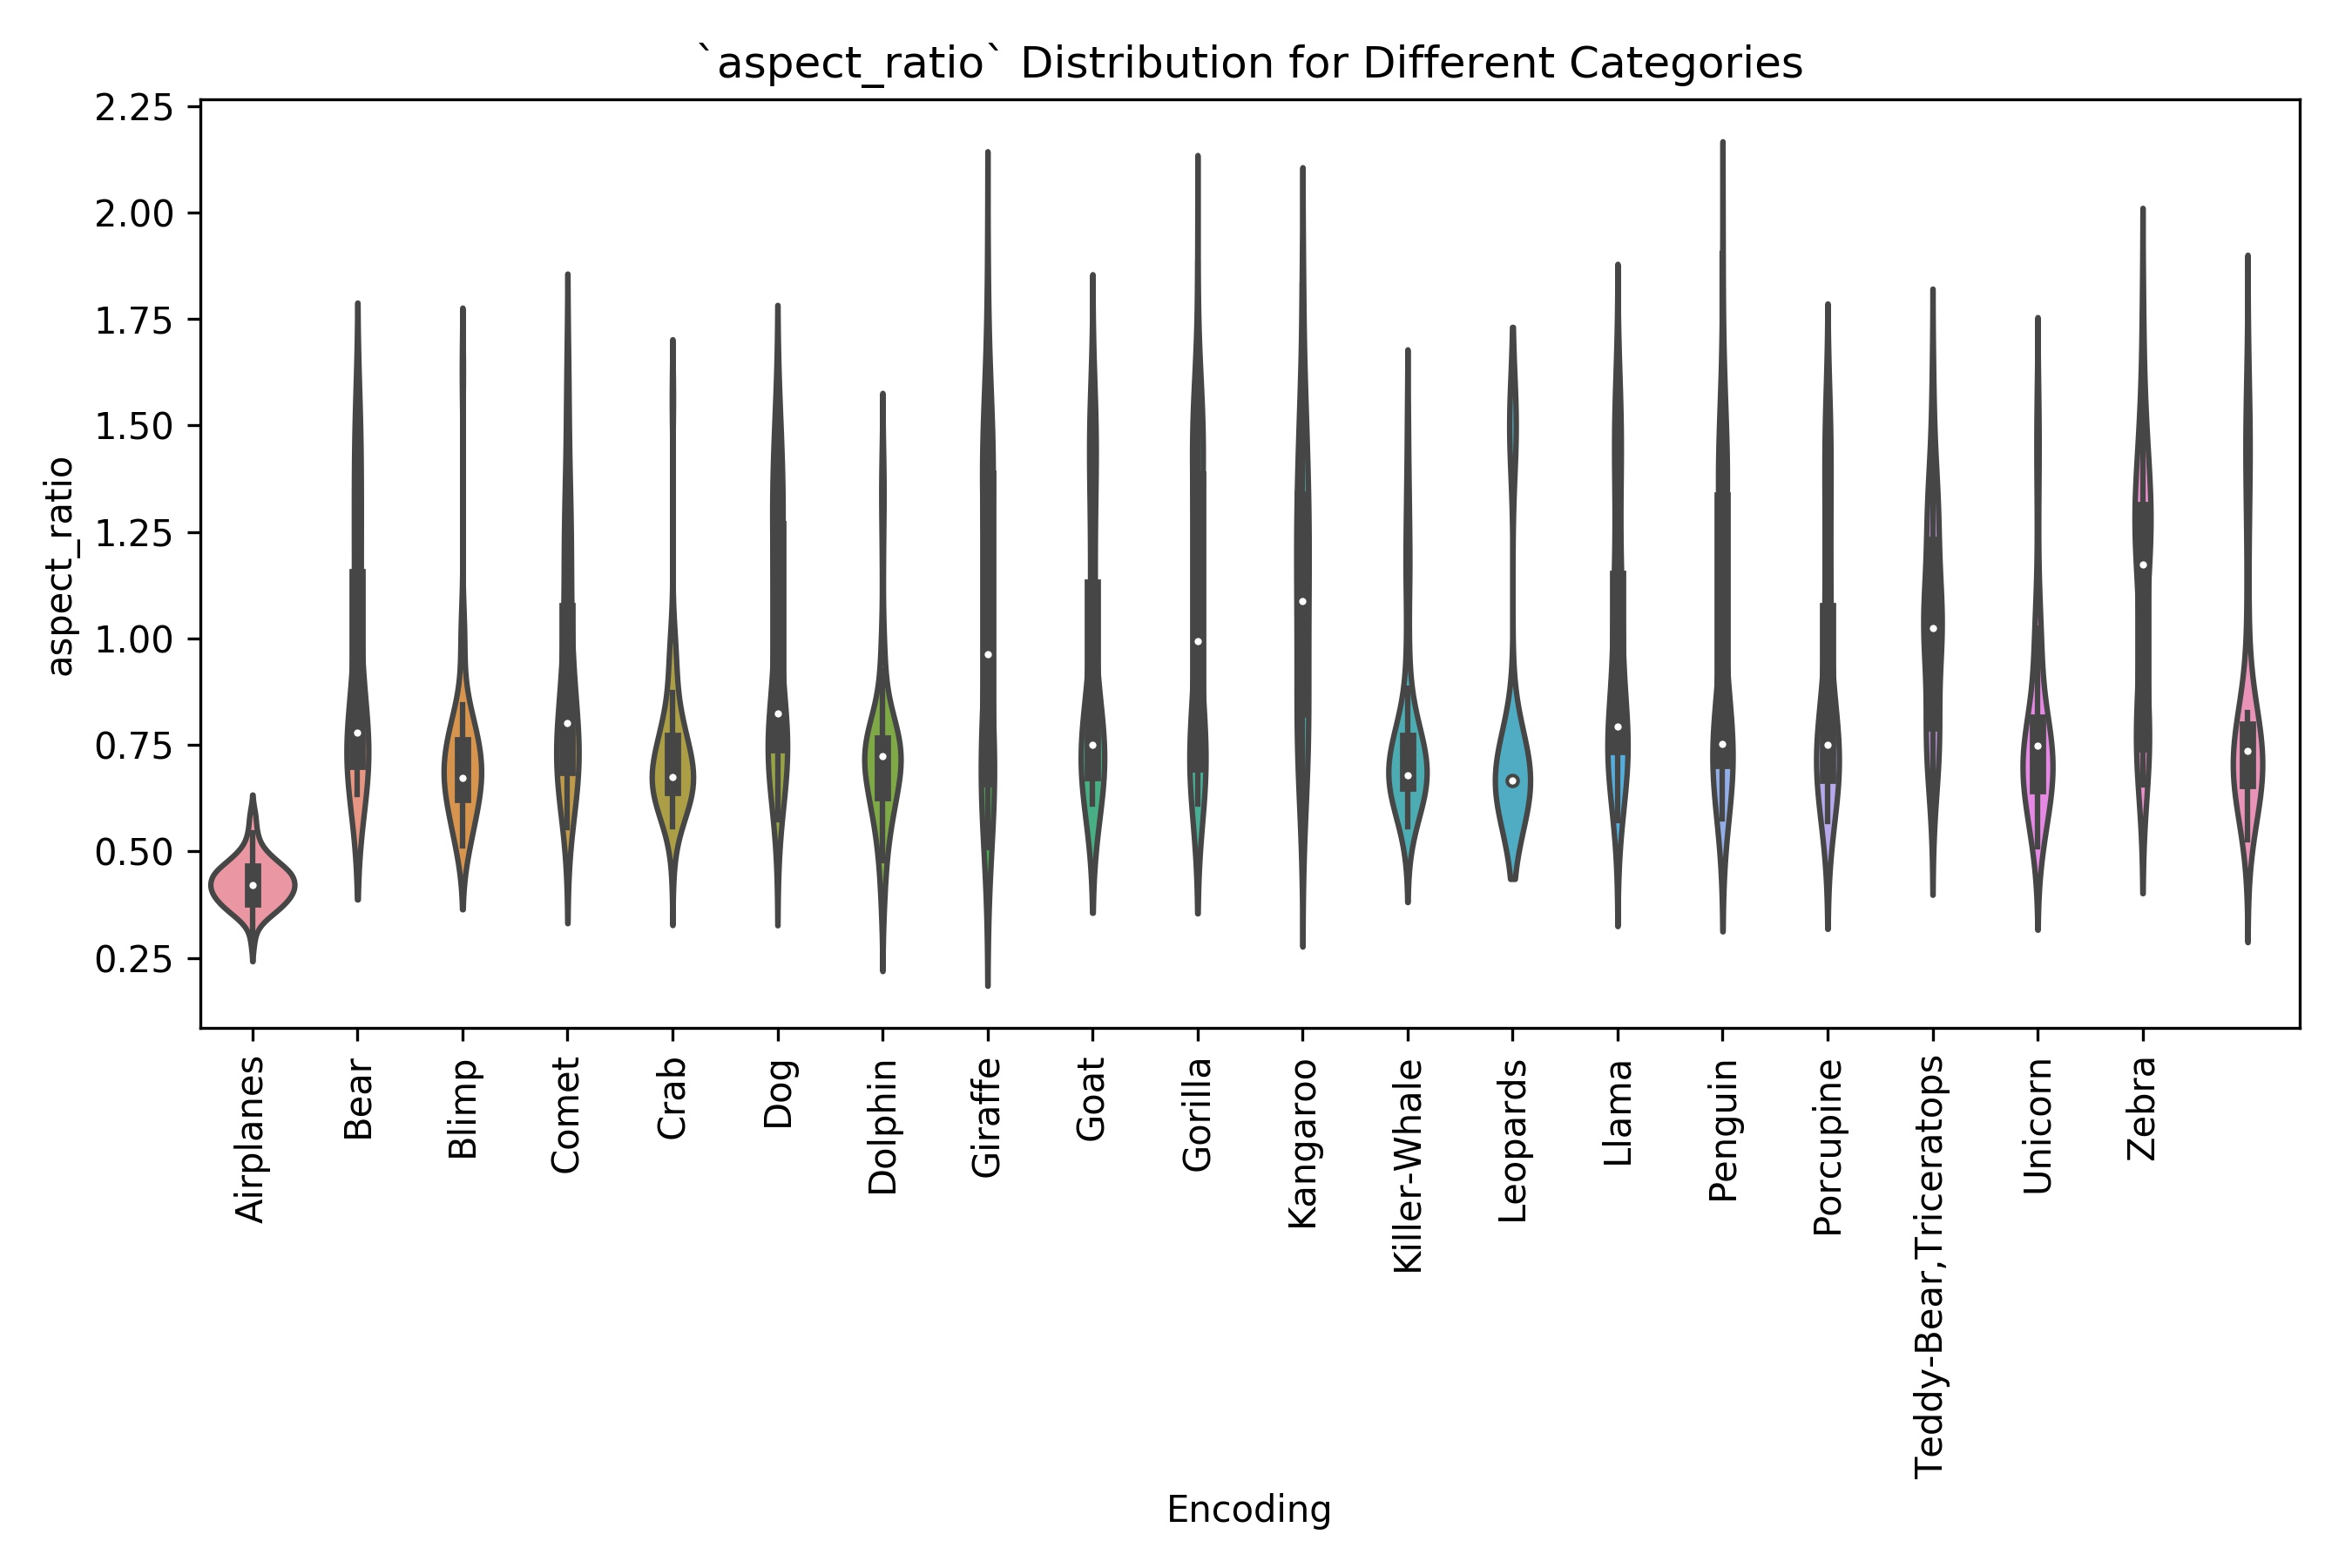
\includegraphics[width=8cm]{image/aspect_ratio.jpg}
\caption{\label{fig:aspect_ratio}EDA of ``aspect\_ratio''}
\end{minipage}
\end{figure}

``avg\_y'' feature of \textit{comet} class has a very different distribution compared with other classes. The average of ``avg\_y'' of \textit{comet} is less than other classes. That's because comet images always have dark backgrounds, resulting in low luminance. 

The distribution of ``aspect\_ratio'' of \textit{airplanes} class is also different from other distributions. That's because airplanes always spread horizontally in training images, thus images containing airplanes are more likely to be flat rectangle pictures with low ``aspect\_ratio''.

Before EDA process, I thought ``harris'' can be a useful feature. For images containing \textit{crabs} and \textit{zebra} can be detected with more harris corners than other classes. However, after visualization, the distributions of different classes are quite similar.

\section*{Model Training}
We tried four models on the dataset, also tuned parameters to get best performance. 90\% of our data was used as training set and 10\% as validation set. In this section, we will walk through each model and dig into the details. It's noteworthy that we fixed all random seeds in training process for easy reproduction.
\subsection*{Logistic Regression}
We started with the simplest model. To prevent overfitting, we added regularization term for logistic regression. We searched L1 and L2 regularization and corresponding hyperparameter. For L2 regularization, we also tested models with different multiclass options (``ocr'' and ``multinomial'').

The best logistic regression model achieved 43.71\% accuracy on validation set and 42.44\% on training set. The hyperparameter set was $C = 10$ and $penalty=$`l1'.

Figure~\ref{fig:lg} is a graph showing performance of logistic regression models with different hyperparameter. We can see that hyperparameter C strongly affects the accuracy. For our best model, the accuracy on validation test is quite similar to training set, showing there is not overfitting.

\begin{figure}[!h]
\centering
\begin{minipage}[t]{0.48\textwidth}
\centering
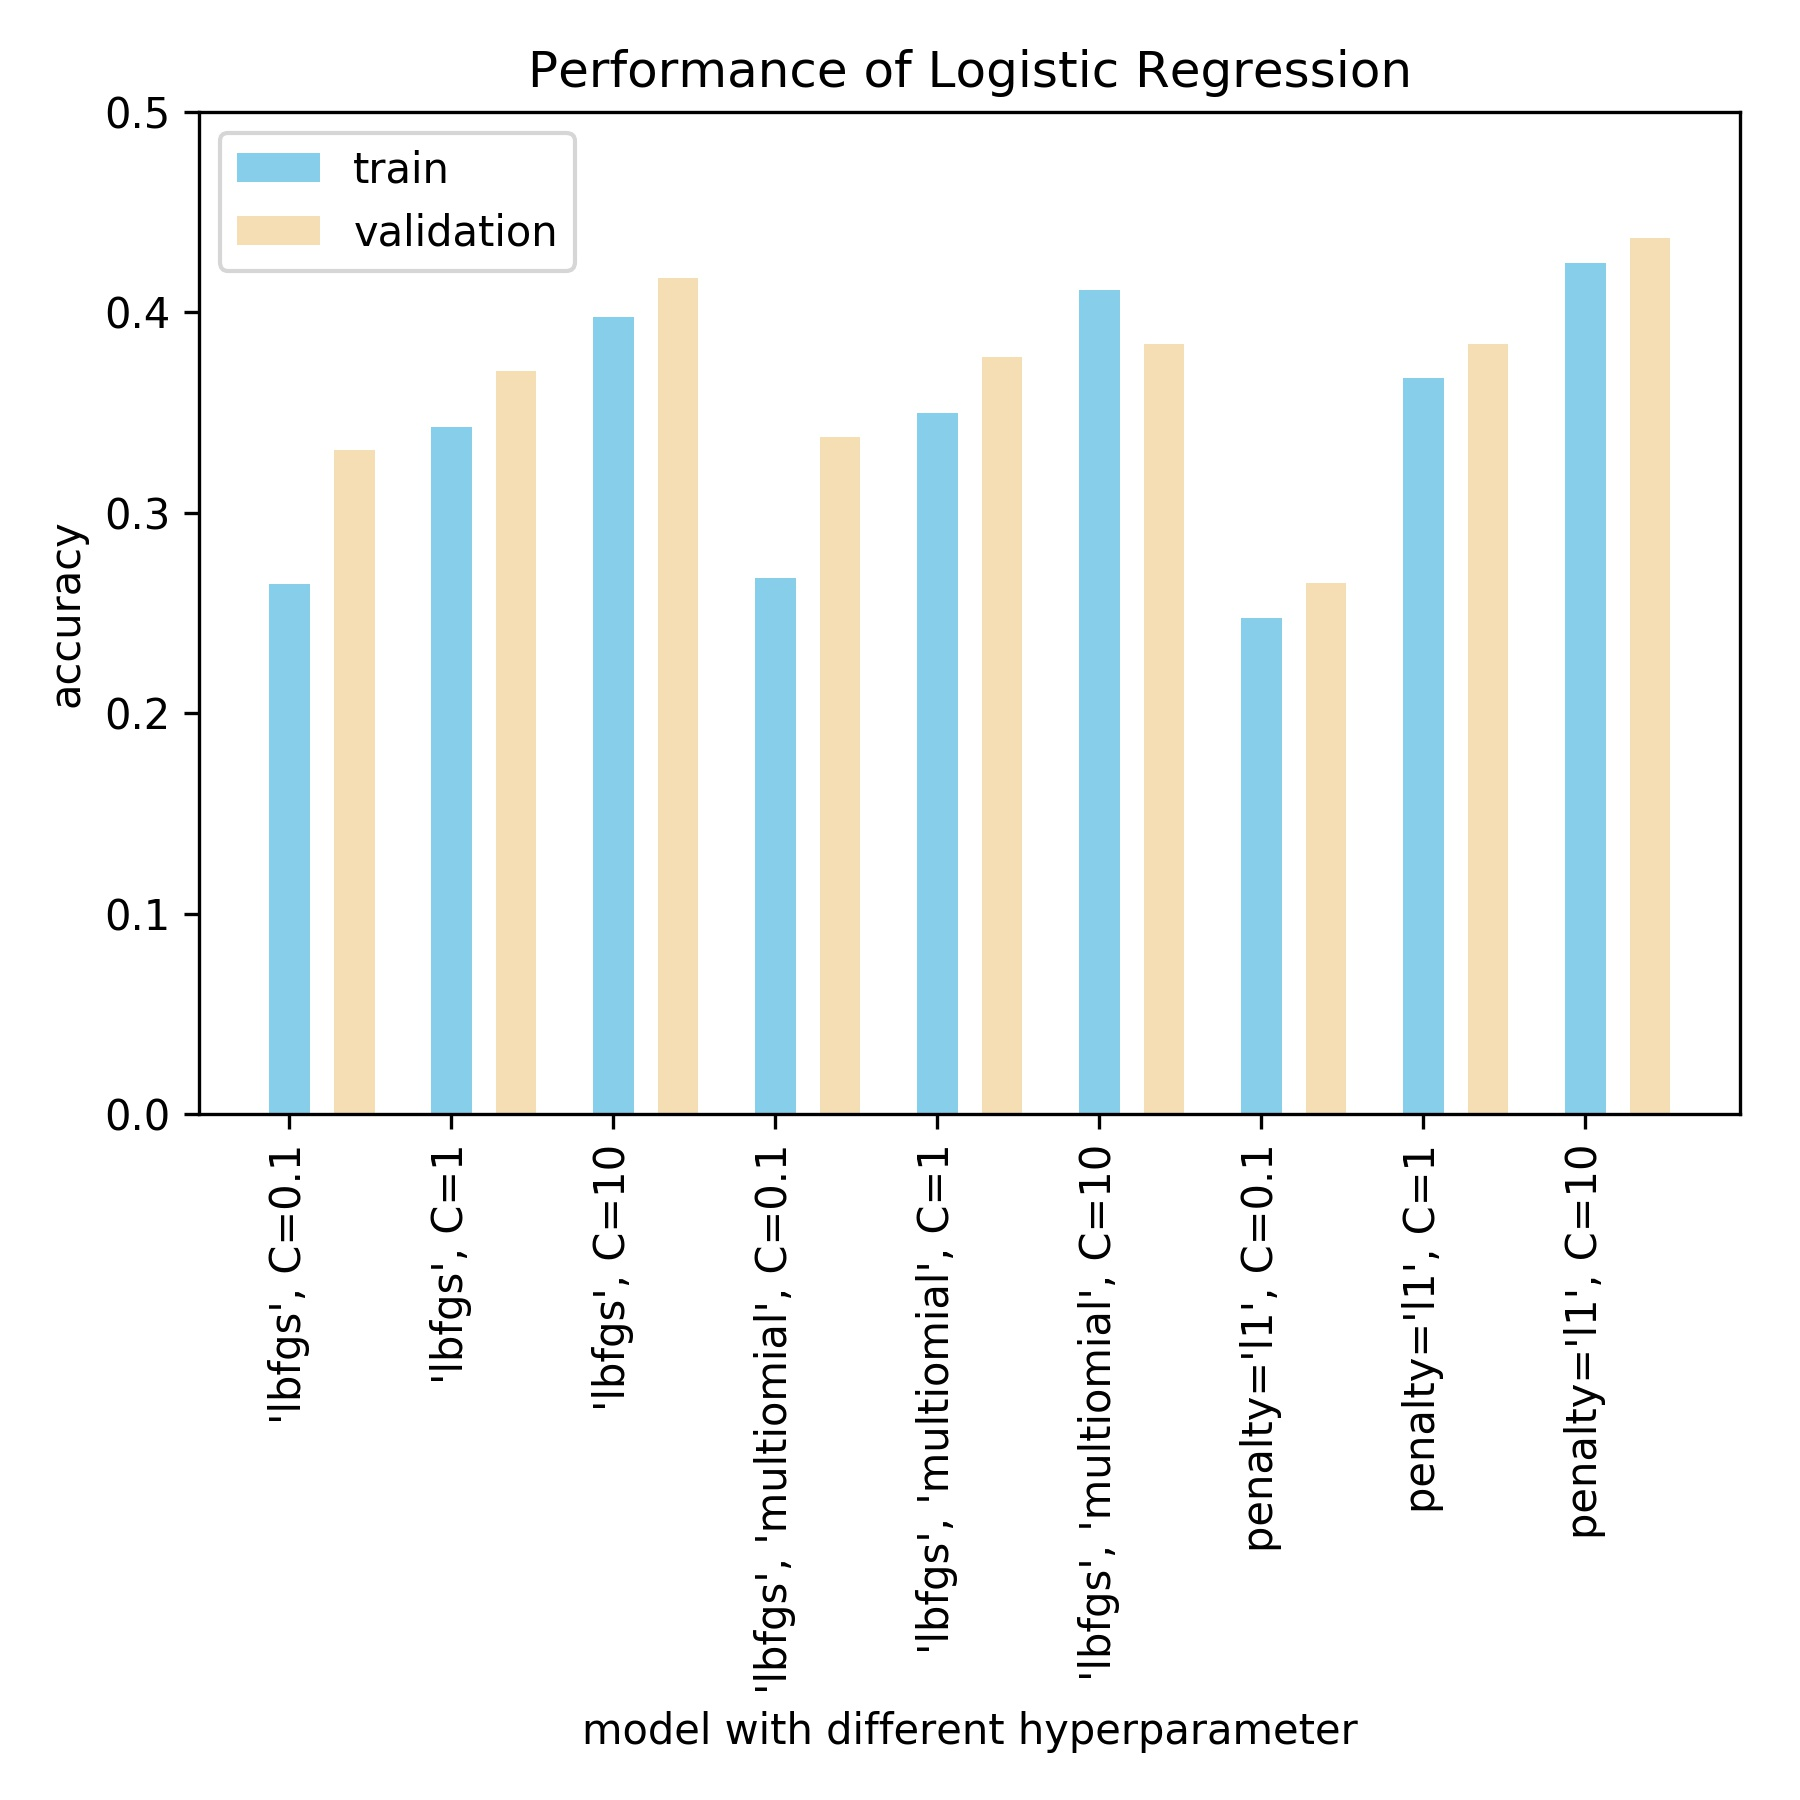
\includegraphics[width=8cm]{image/lg.jpg}
\caption{\label{fig:lg}Performance of Logistic Regression}
\end{minipage}
\begin{minipage}[t]{0.48\textwidth}
\centering
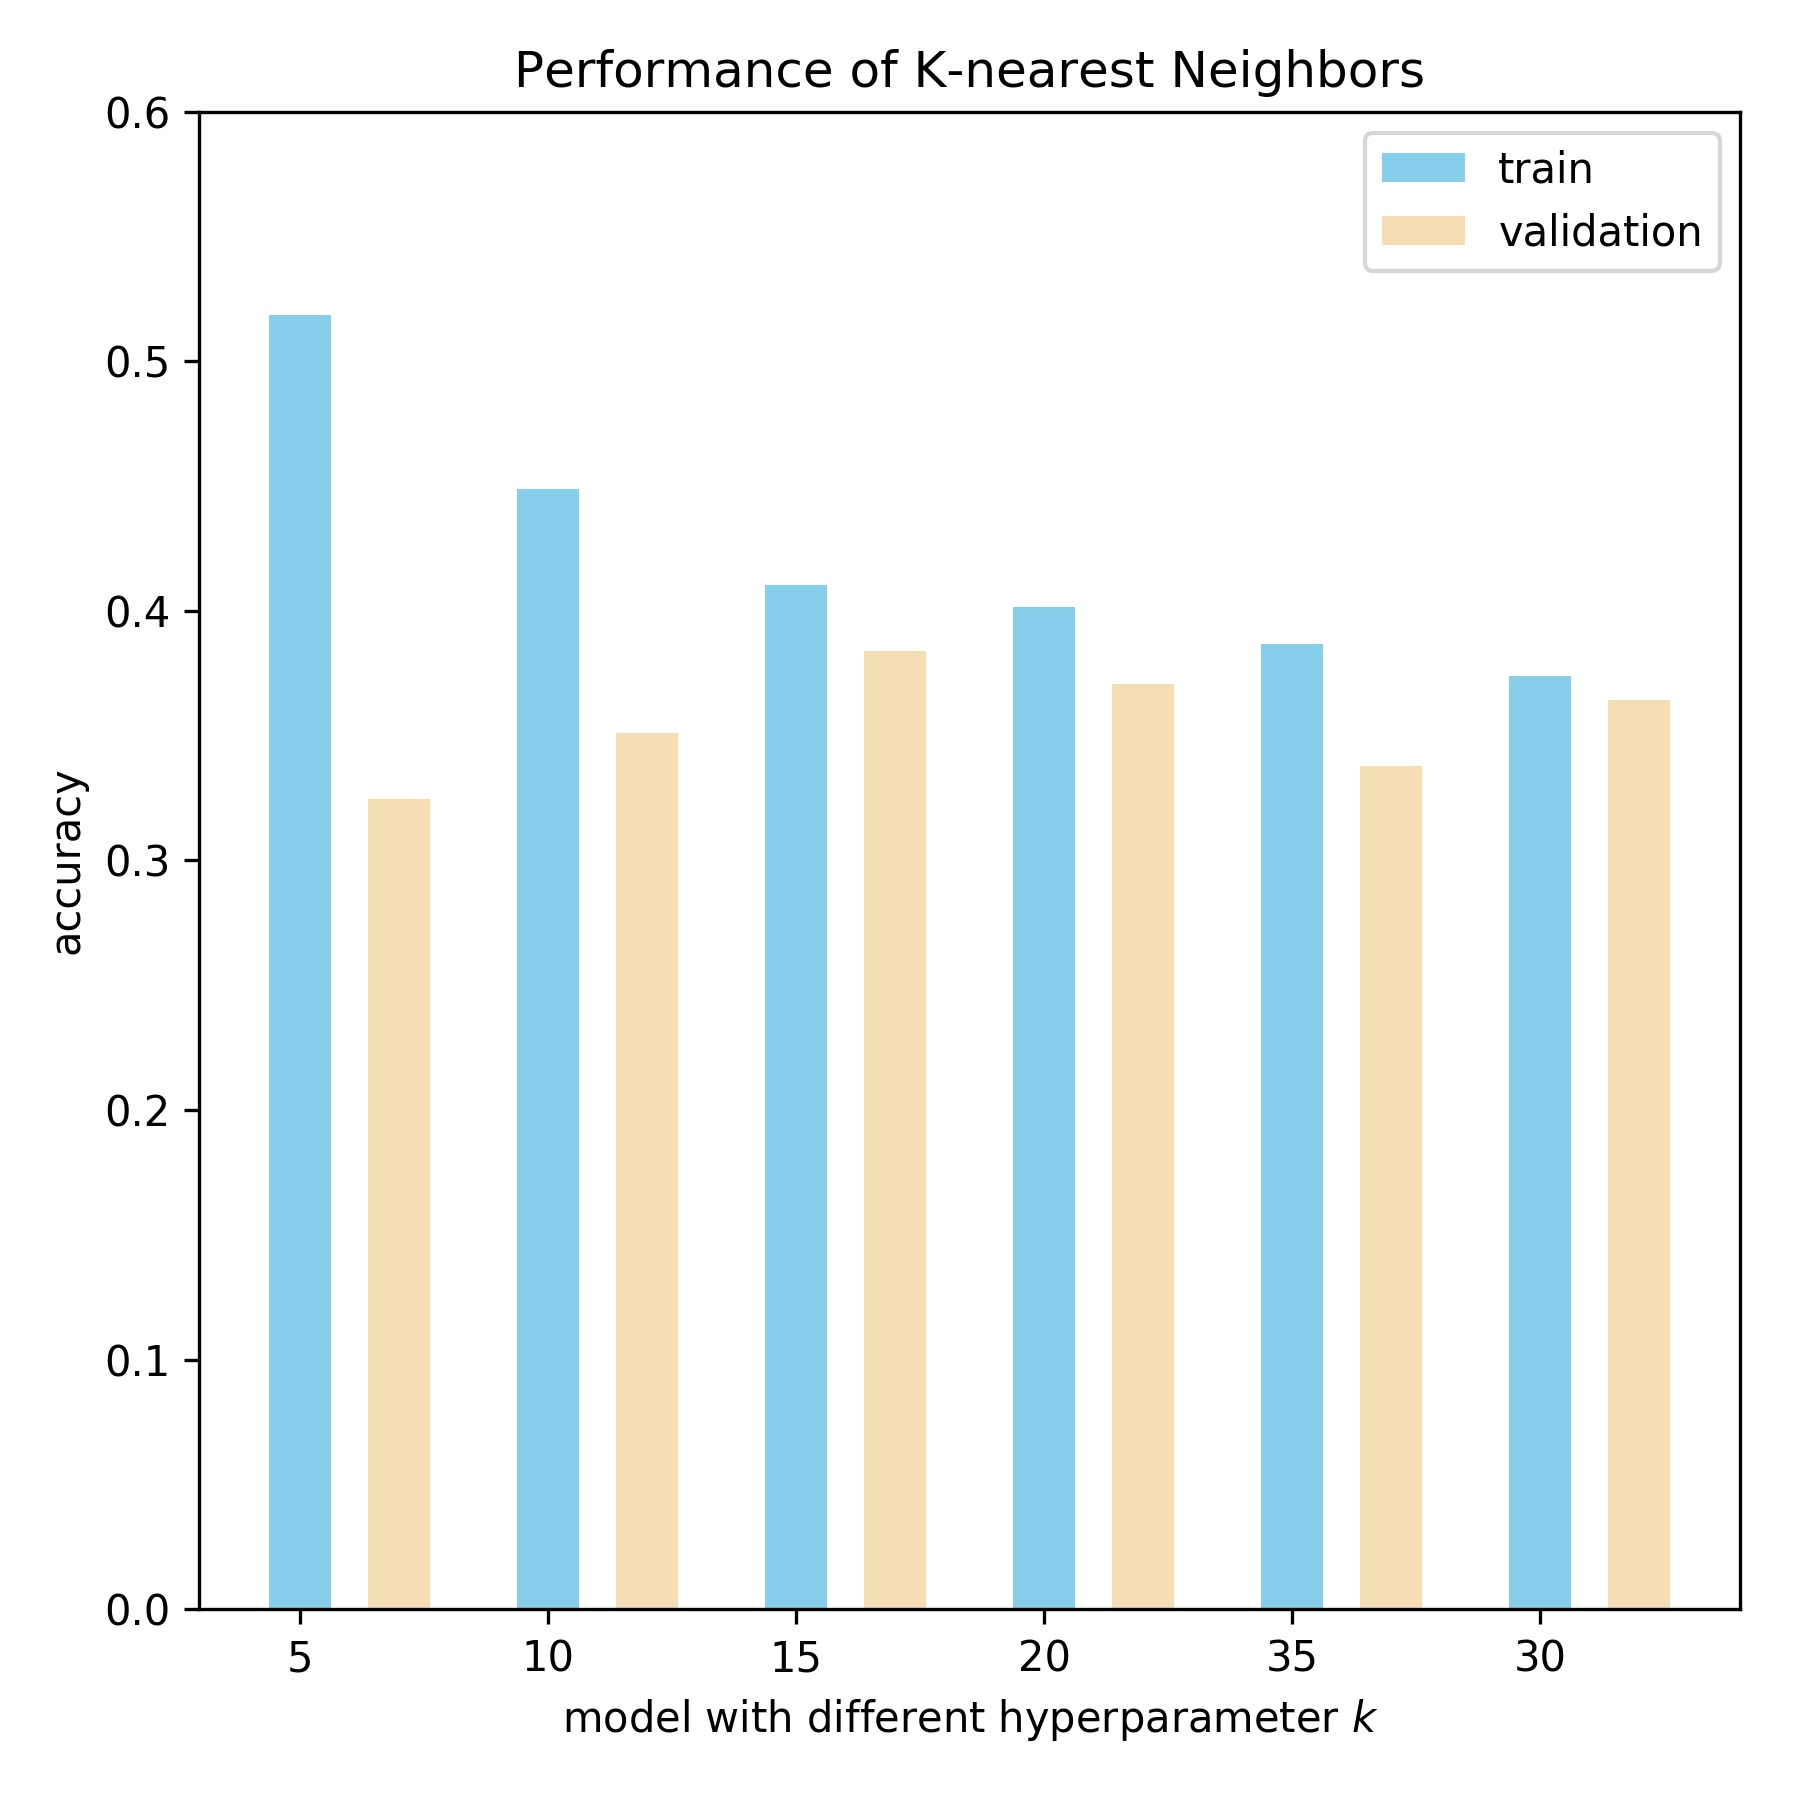
\includegraphics[width=8cm]{image/knn.jpg}
\caption{\label{fig:knn}Performance of K-nearest Neighbors}
\end{minipage}
\end{figure}

\subsection*{K-nearest Neighbors}
KNN is a non-parametric method for classification. We can classify a image by a majority vote of its neighbors in feature vector space. The image will be assigned to the class which is most common among the image's k nearest neighbors. We tried different parameter of $k$ to search for best model.

The best k-nearest neighbors model achieved 41.03\% accuracy on validation set and 38.41\% on training set, with parameter $k = 5$.

Figure~\ref{fig:knn} is a graph showing performance of k-nearest neighbors models with different parameter $k$. As $k$ becomes large, the accuracy of training set decreases, showing that it's easy to overfit when $k$ is small. This may be caused by lack of data. However, the accuracy on validation test doesn't fluctuate as much as training accuracy when $k$ changes.

\subsection*{Random Forest}
Random forests are an ensemble method for classification by constructing a forest of decision trees during training. The output of random forest model is the mode of the classes of the individual decision trees. We tried models with different parameter `n\_estimators' and `max\_depth'. The first parameter represents the tree number in random forest and the second stand for maximum depth in an individual tree.

The best random forest model achieved 48.67\% accuracy on validation set and 41.06\% on training set. The best parameter set is $n\_estimators = 100, max\_depth = 6$.

Figure~\ref{fig:rf} showing performance of k-nearest neighbors models with different parameters. As `max\_depth' increases, the accuracy of training set goes up significantly, indicating that random forest can easily overfit. 

\begin{figure}[!h]
\centering
\begin{minipage}[t]{0.48\textwidth}
\centering
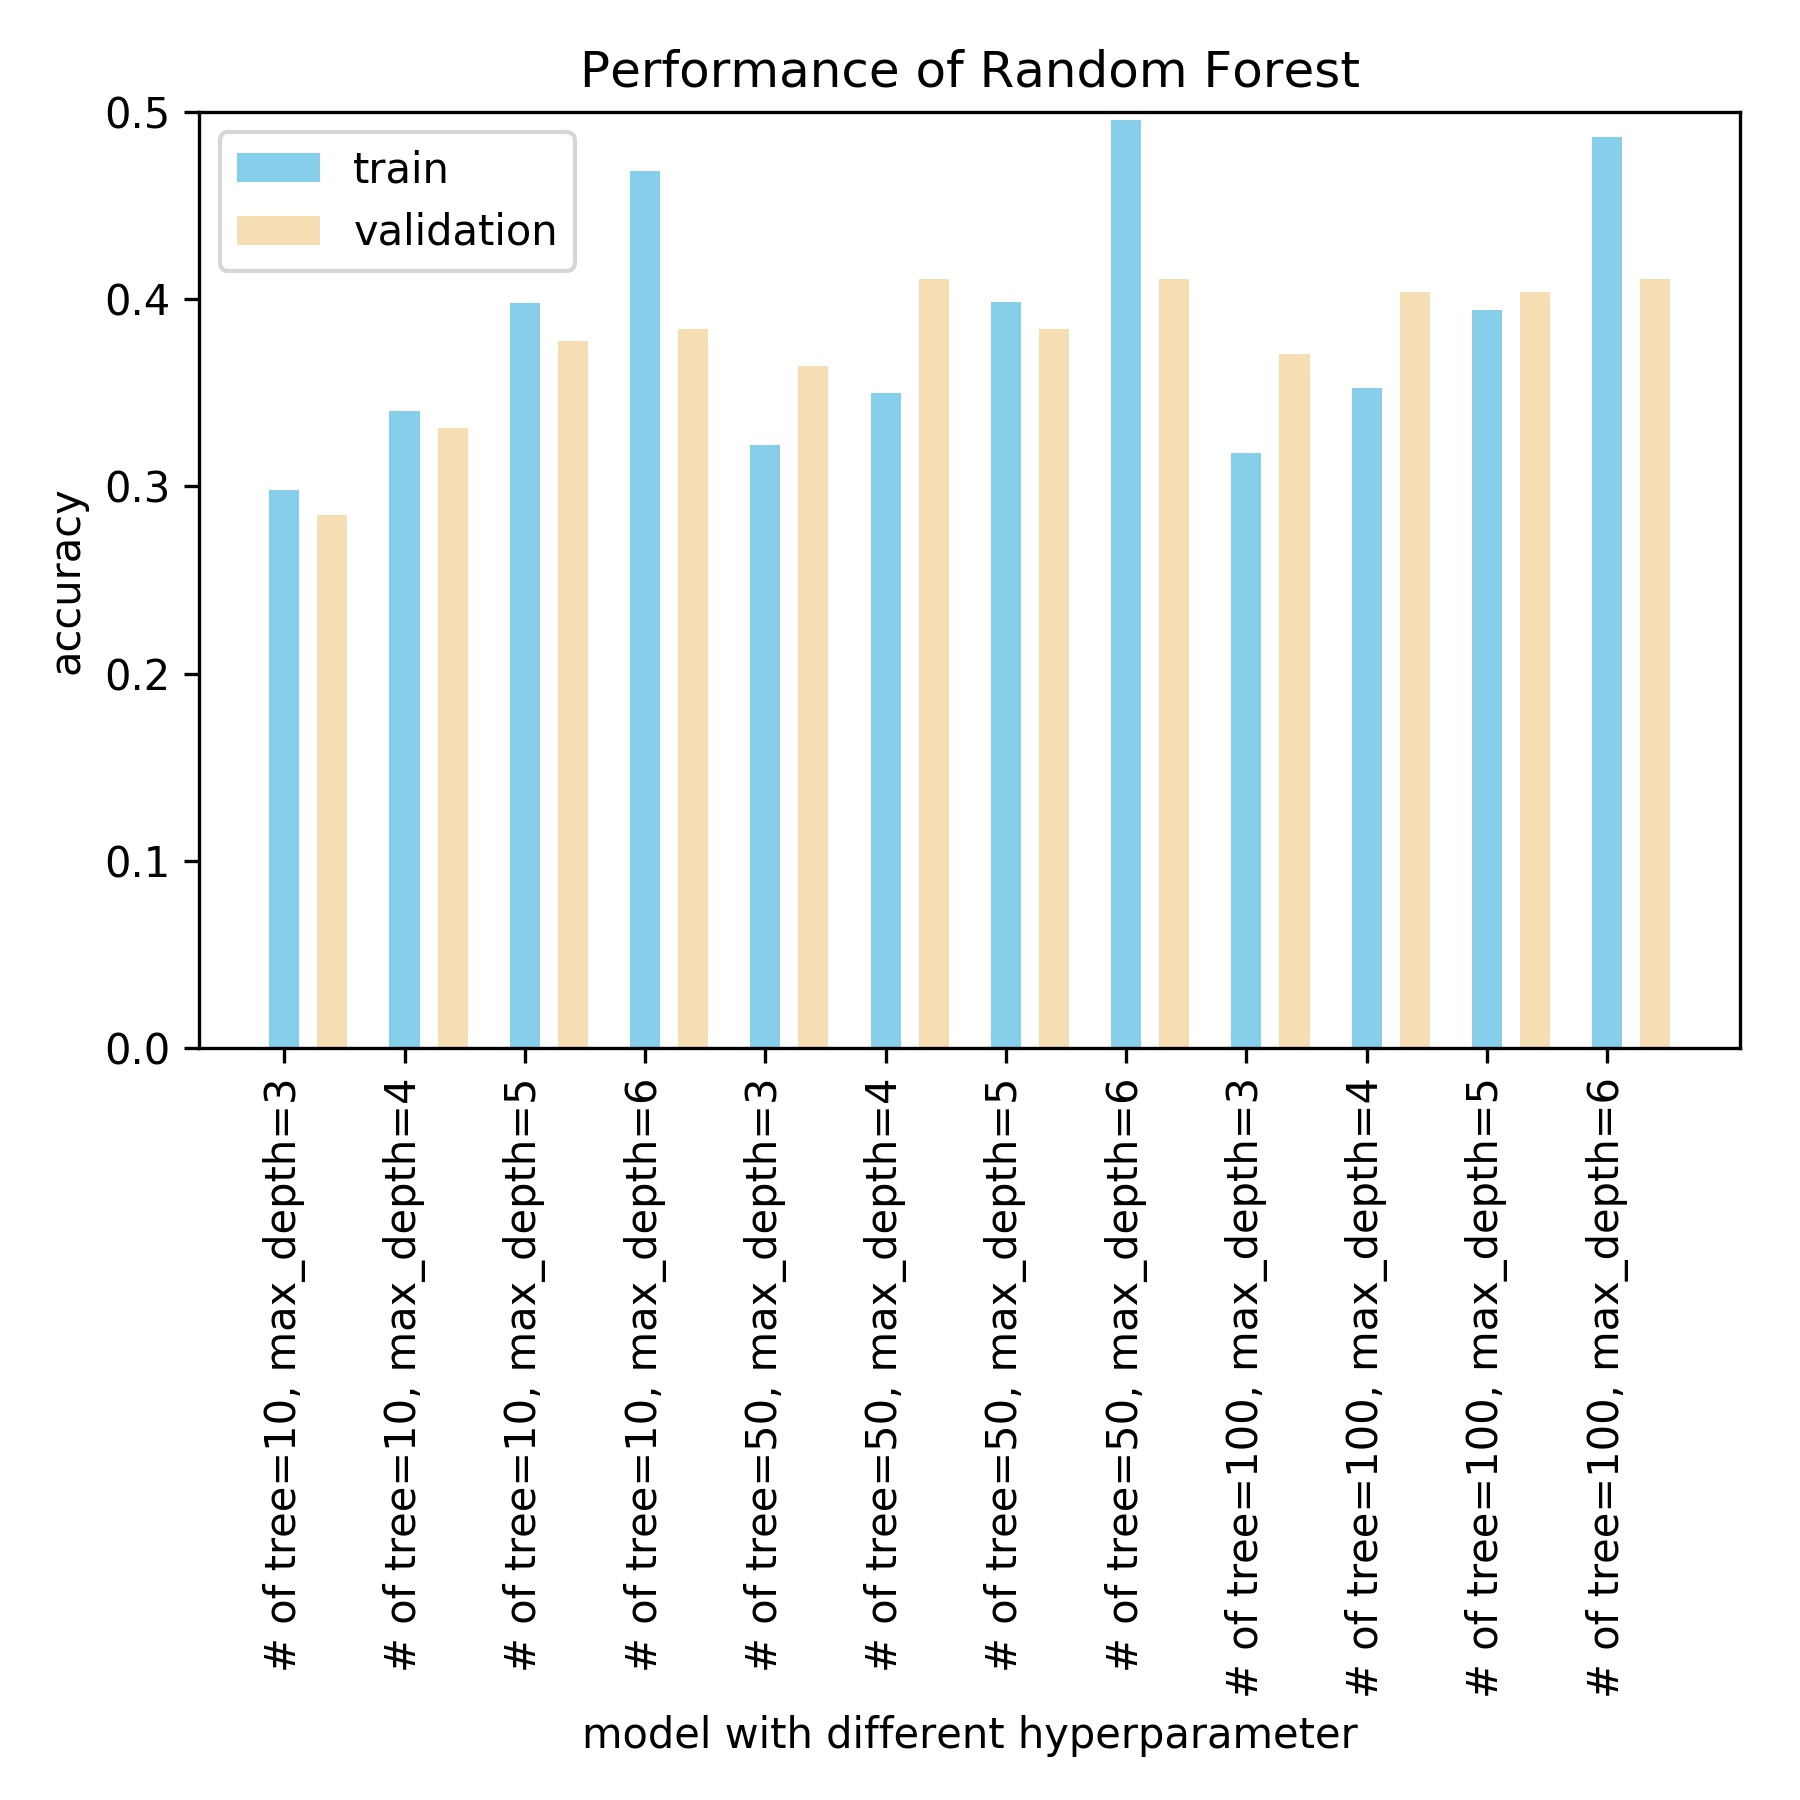
\includegraphics[width=8cm]{image/rf.jpg}
\caption{\label{fig:rf}Performance of Random Forest}
\end{minipage}
\begin{minipage}[t]{0.48\textwidth}
\centering
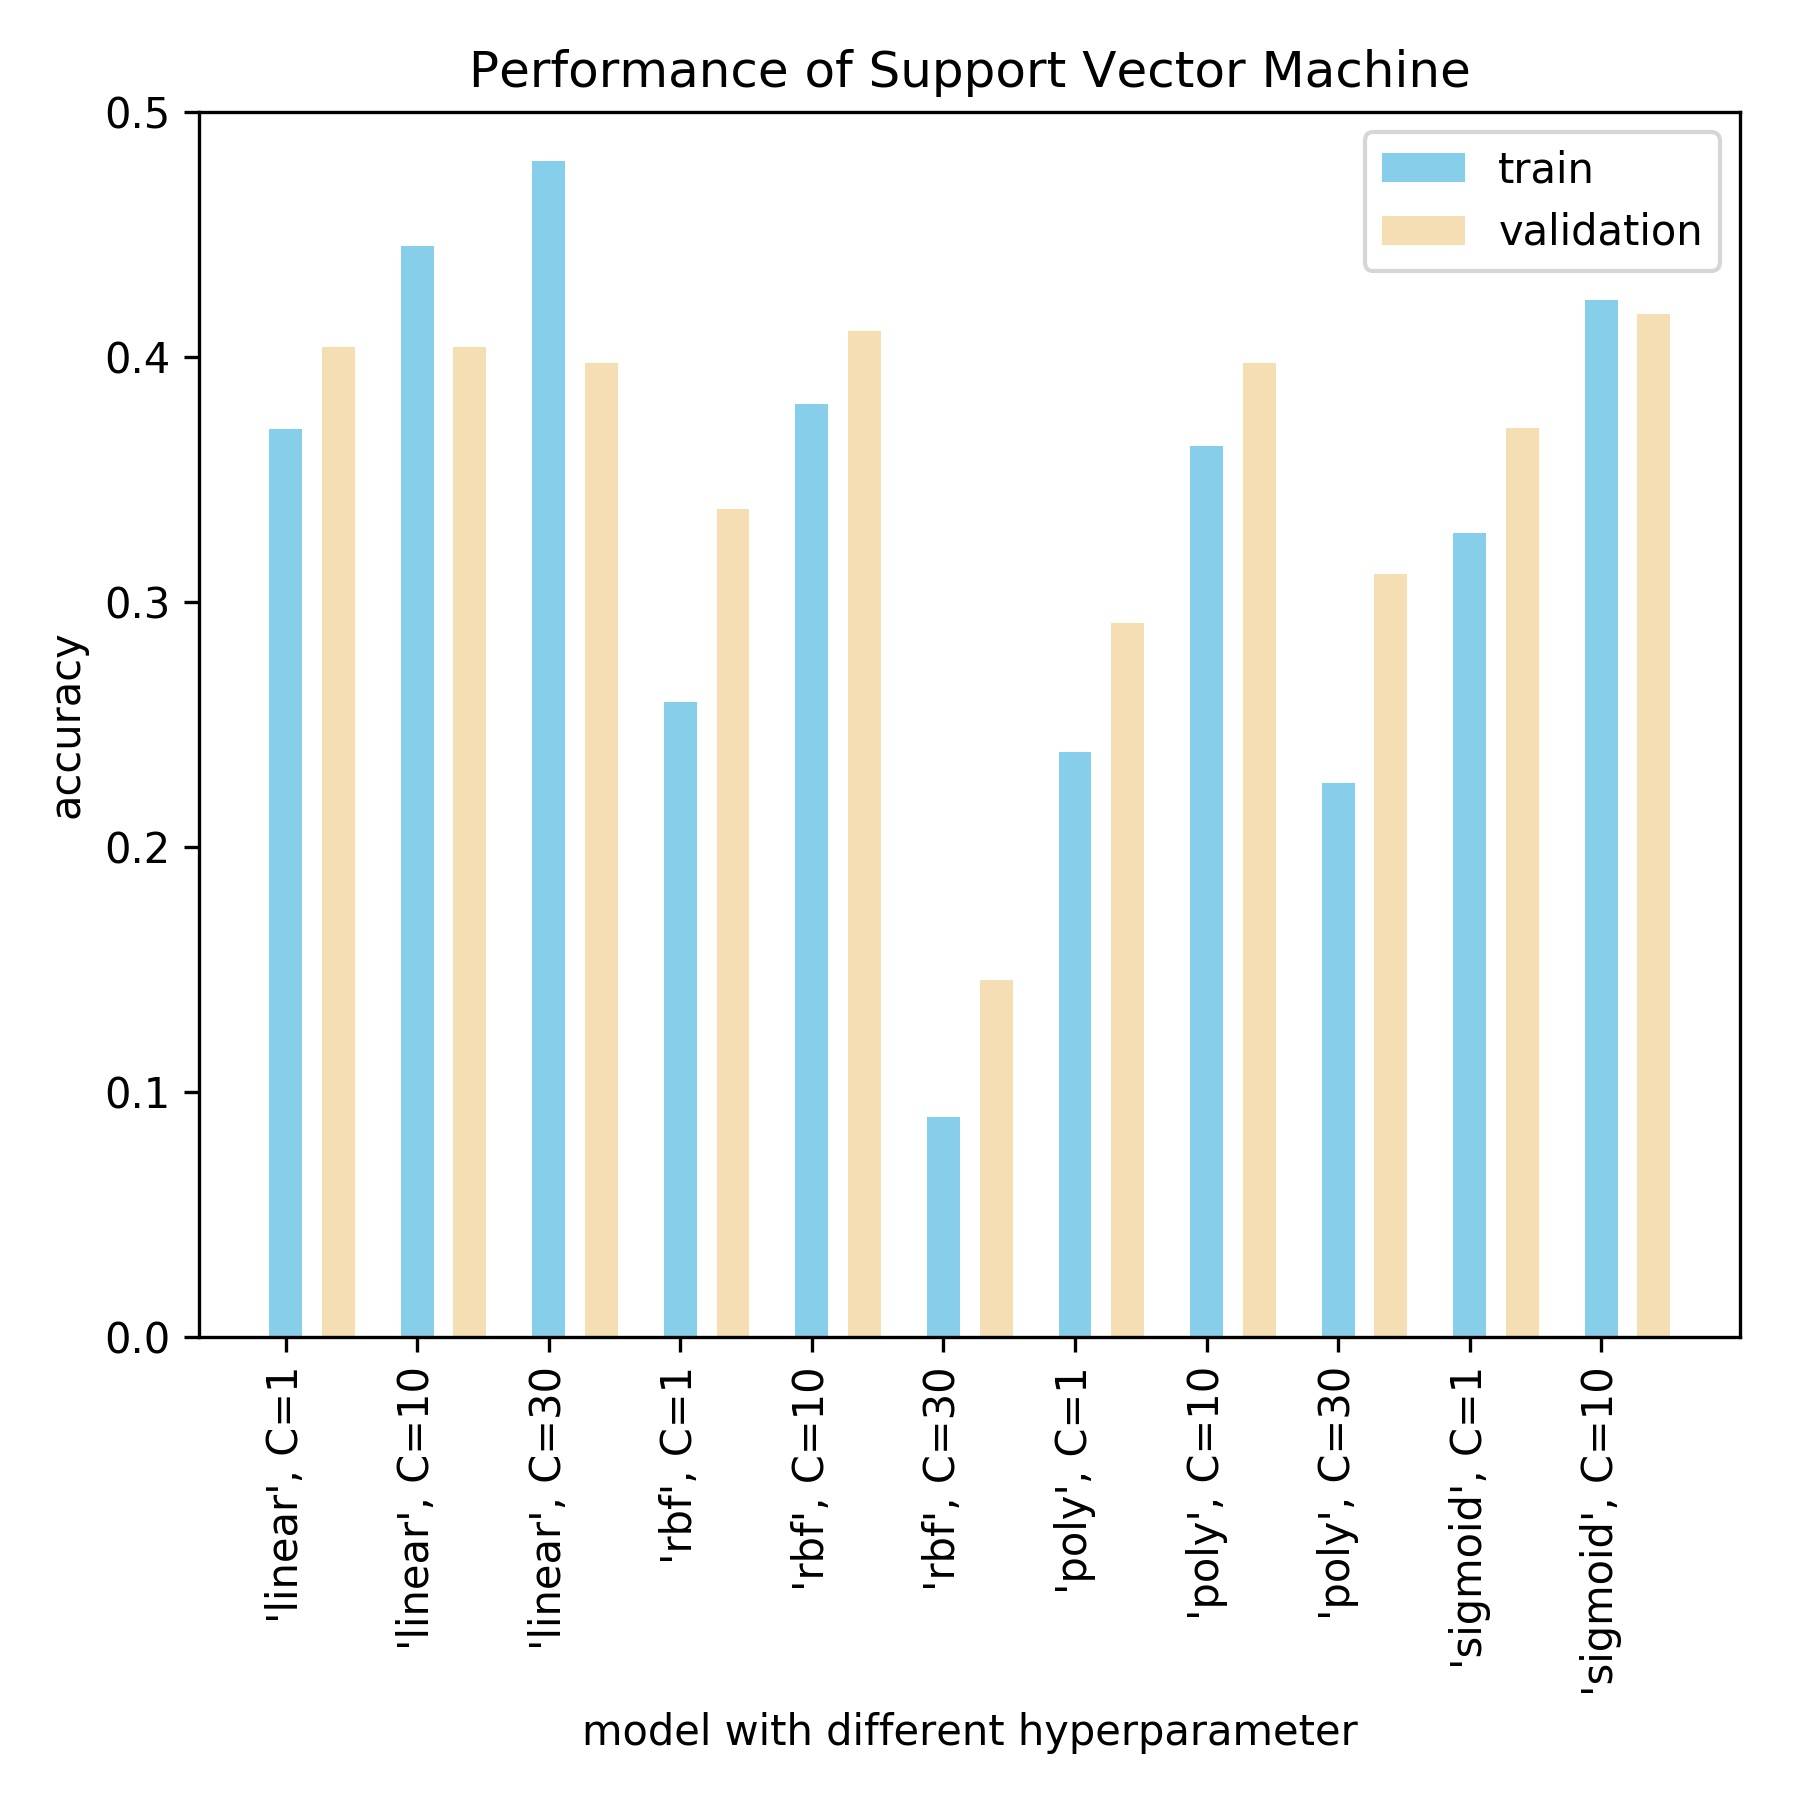
\includegraphics[width=8cm]{image/svm.jpg}
\caption{\label{fig:svm}Performance of Support Vector Machine}
\end{minipage}
\end{figure}

\subsection*{SVM}

We also employed support vector machine model on our dataset. We tried 4 kernel function: `lilnear', `rbf', `poly' and `sigmoid' with different penalty terms.

The best support vector machine model achieved 41.72\% accuracy on validation set and 42.30\% on training set, using `sigmoid' kernel anc $C=100$.

Figure~\ref{fig:svm} showing performance of support vector machine models with different parameter set. For very large penalty parameter C, the optimization will choose a smaller-margin hyperplane to do a better job of getting all the training points classified correctly. 

\section*{Tensorflow}
Following the baisc idea of \cite{krizhevsky2012imagenet}, we adopted the deep learning method for image classification with tensorflow. Specifically, we propose to use a CNN-based neural network (3 layer of convolution layer to extract the feature directly from the 3 channels of each image and 3 layer of fully connect network to aggregate the features from the previous layers.) We also resize each image to (224, 224) and scale down each pixel in the range of [0, 1] for numeric stability. The best performance of TF-based model was 41.44\% on training and 39.06\% on validation in terms of accuracy with train/validation split ratio as 9:1.

One thing we find interesting with training of the huge amount of parameters-based NN model is that the regularization seems to help a lot in the generalizability of this model. With the same model structure we described above, we trained the NN with adding 0.0001 scaled regularization to the last 3 fully connected layers and vice versa. We can notice from the following plots, which indicate with regularization the model turns to perform uniformly on both training and validation set. While the model without last three regularization-based layer turns out to enlarge the discrepancy between training and validation, which is known as the `overfitting' issue we have learned from the class. One possible reason for that is the regularization constrained the scale of parameters and make the model more invariant towards small fluctuation of features.
\begin{figure}[!h]
\centering
\begin{minipage}[t]{0.48\textwidth}
\centering
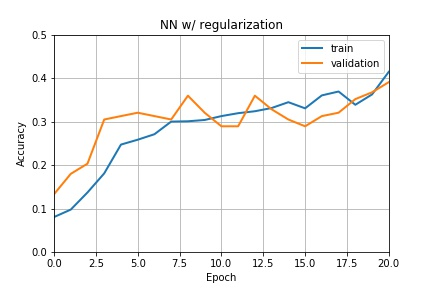
\includegraphics[width=8cm]{image/NNwr.jpg}
\caption{Performance of NN with regularization}
\end{minipage}
\begin{minipage}[t]{0.48\textwidth}
\centering
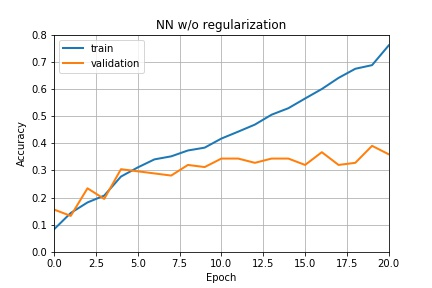
\includegraphics[width=8cm]{image/NNwor.jpg}
\caption{Performance of NN without regularization}
\end{minipage}
\end{figure}


Moreover, for comparison with the ML-based model, we can notice the advantage of NN is that the larger amount of parameters actually makes it capable of fitting any kinds of function, but also accompanies the potential risk of more likely to `overfitting'. On the other hand, ML-based model turns out to be more stable (small variations) but less capable of fitting dataset. One possible future direction is to extract the feature from the last layer of NN and feed that into ML-based model, which might thus combine the advantage of both models.

\section*{Conclusion}
The multi-class classification of images is possible through machine learning and computer vision algorithms. One of the biggest pain point we drew from the project is the wide varieties of possible data (inequality of labelled training data will easily lead to overfitting in that class). Therefore, in order to further create a more accurate system, there needs to be a large and continuously growing data source. Moreover, we discover the different advantages of ML and DL-based models and point out a possible direction for future system design in image detection.

\bibliography{ref}{}
\bibliographystyle{plain}
\end{document}
